\bisection{绪论}{Introduction}
本模板根据中国矿业大学硕士研究生毕业论文模板要求进行编写,下面将重点介绍本模板的使用方式,基础使用方式将不再介绍。\par
使用\LaTeX 编写论文的方便之处此处不再过多赘述,相信大家在使用的过程中会有很深的体会,需要注意的一点是,部分查重平台由于其PDF识别程序的问题,会导致无法识别他引率,如维普,笔者经过多次测试发现,其原因在于,在识别PDF文件时,会将引用上角标的左侧中括号识别成和前一个字符相同的字节长度,通俗来讲即,引用上角标如果放在中文后面,引用上角标的左侧中括号将会是一个全角的中括号,这与引用格式不同,故而无法识别他引率,解决该问题的办法之一即是将引用上角标放在英文或者数字的后面,该问题已向维普官方的反馈,官方表示将在后面两个版本中对该问题进行优化。
\bisubsection{编译器}{Compiler}
本模板上传至Overleaf的模板库供大家使用,Overlaef是\LaTeX 在线编辑工具,具有强大的命令补全功能,需要注意的是Overleaf模板库中下载的模板已在Overleaf中调试完成,在其他平台下载到的资源不能直接导入Overleaf中使用。此外,本模板还将上传至Github、\LaTeX 工作室等多个平台供大家使用本地编辑器使用,比如TeX Studio。

\bisubsection{标题}{Headings}
\subsubsection{一级与二级标题}
根据中国矿业大学硕士毕业论文模板要求,一级与二级标题需要同时使用中英文标题,其样式如图(\ref{fig:headings})所示。\par 
\begin{figure}[htbp]
	\centering
	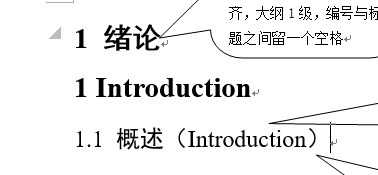
\includegraphics{pictures/headingsStyle.png}
	\bicaption{一级与二级标题样式示意图}{Schematic diagram of primary and secondary headings styles}
	\label{fig:headings}
\end{figure}
本模板定义了生成上图格式的一级(\verb|\bisection{中文标题}{英文标题}|)与二级标题(\verb|\bisubsection{中文标题}{英文标题}|)命令。不同于只生成单标题的一级(\verb|\section{中文标题}|)与二级标题(\verb|\subsection{中文标题}|)命令,前面两个命令将同时可以自动生成对应的中英文目录。其余关于段落标题的命令将不变。

\bisubsection{图表}{Figures and tables}
\subsubsection{双语图表名称}
如果想要生成中英文的图和表的名称,将需要使用\verb|\bicaption{中文标题}{英文标题}|,该命令将同时自动生成图表的中英文清单,样式如图(\ref{fig:f-tN})所示。如果只使用\verb|\caption{标题}|命令将只会得到单个标题,同时图表清单上面也只会显示一个标题条目\ref{fig:fn}。\par
\begin{figure}
	\centering
	\subfigure[]{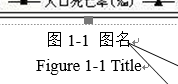
\includegraphics[width = .5\textwidth]{pictures/figureName.png} \label{fig:fn}}
	\subfigure[]{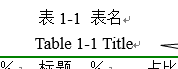
\includegraphics[width = .5\textwidth]{pictures/tableName.png}\label{fig:tn}}
	\bicaption{\subref{fig:fn}图片名称样式;\subref{fig:tn}表格名称样式}{\subref{fig:fn} Style of figure name;\subref{fig:tn} Style of table name}
	\label{fig:f-tN}
\end{figure}
\subsubsection{表格线}
中国矿业大学硕士毕业论文模板中所给的表格线颜色为绿色,虽未明确说明,但在本模板中还是给出了该线颜色的命令,只需要在表格中第一处需要添加表格线的命令前面加入\verb|\arrayrulecolor{tablinecolor}|命令即可将该表格中的线变成绿色。

\bisubsection{信息}{Information}
本模板定义了三种命令来帮助我们生成封面等部分信息,分别是\verb|\title{中文题目}{英文题目}|、\verb|\infor{作者}{指导老师(加职称)}{工学硕士学位}{化工学院}{学科专业}{研究方向}| 、\\ \verb|\Time{年}{月}{汉字年份(二〇二三)}{汉字月份(三)}|。

\bisubsection{模板结构}{Template structure}
本模板包含.tex 、.cwl 、.bib 、 .clc等文件以及fonts、logo、picture、SectionTeX文件夹。为了方便管理论文,该模板结构采用章节分开的方式进行管理,.tex文件中包含了整个论文的框架,SectionTeX文件夹中包含了各个章节的.tex文件,作者只需要将在SectionTeX文件夹中存在的章节文件在根目录下的.tex文件的适当位置使用\verb|\input{}|命令即可。.bib文件中存放的是参考文献的信息。.cls文件即为该模板的样式文件,非必要不修改!!!.cwl文件中写入的是新定义的命令,可在命令补全时显示作用。SectionTeX文件夹中写入了一些必要的章节,如abstract.tex为摘要部分,作者需要将中英文摘要写入该文件中,thank.tex为致谢章节,作者需要将致谢部分写入该文件中,contenttabs.tex文件里面包含了生成目录以及图表清单、以及变量注释表的必要命令,除变量注释表之外无需作者更改,变量注释表采用环境的方式给出,该环境已经封装了长表格环境,作者仅需将每一行的条目写入即可,introduction.tex为绪论章节,作者可将绪论这一章的内容写入该文件中,conclude.tex为结论章节,作者可将结论这一章的内容写入该文件中,reference.tex为生成参考文献的命令内容,无需作者更改,resume.tex为作者简介章节,作者需要将个人简历写入该文件中,appendix.tex、declaration.tex、dataCollection.tex分别为附录、声明以及数据集。其他章节文件作者可以自行新建,如果内容较少也可以将若干章的内容写入同一个文件中\footnote{在需要使用脚注的地方使用{ \texttt{\char92} footnote\{脚注内容\}}命令可以生成脚注。}。

\begin{figure}[htbp]
	\centering
	
\includegraphics[width=0.8\textwidth]{{logo/zgkydx_logo}}
	\bicaption{中国矿业大学logo}{zgkydxlogo}
\end{figure}

\begin{figure}[htbp]
	\centering
	
\includegraphics[width=0.8\textwidth]{{logo/zgkydx_logo}}
	\bicaption{中国矿业大学logo}{zgkydxlogo}
\end{figure}

\begin{table}[H]
	\renewcommand\arraystretch{1}
	\centering
	\setlength{\abovecaptionskip}{10pt}
	\setlength{\belowcaptionskip}{0pt}
	\bicaption{这是一个普通表格}{Table}
	\label{table2}  
	\begin{tabular}{p{0.4\textwidth}<{\centering}p{0.4\textwidth}<{\centering}}
		\toprule[1.5pt]
		列1 & 列2\\
		\toprule[1.5pt]
		1&\multirow{2}{*}{6}\\
		3&\\
		5&6\\
		\toprule[1.5pt]
	\end{tabular}
\end{table}

\begin{table}[H]
	\renewcommand\arraystretch{1}
	\centering
	\setlength{\abovecaptionskip}{10pt}
	\setlength{\belowcaptionskip}{0pt}
	\bicaption{这是一个普通表格}{Table}
	\label{table1}  
	\begin{tabular}{p{0.4\textwidth}<{\centering}p{0.4\textwidth}<{\centering}}
		\arrayrulecolor{tablinecolor} 
		\toprule[1.5pt]
		列1 & 列2\\
		\toprule[1.5pt]
		1&\multirow{2}{*}{6}\\
		3&\\
		5&6\\
		\toprule[1.5pt]
	\end{tabular}
\end{table}

